\documentclass{beamer}
\usepackage[ngerman]{babel}
\usepackage[utf8x]{inputenc}
\usepackage{ucs}
\usepackage{amsmath}
\usepackage{amsfonts}
\usepackage{amssymb}
\usepackage{pgfpages}

\pgfpagesuselayout{resize to}[a4paper,landscape]

% Style
\usetheme{Bergen}
\usecolortheme{beetle}

\setbeamertemplate{footline}[frame number]
\beamertemplatenavigationsymbolsempty
\setbeamercovered{transparent}

\author{Ferdinand Niedermann und Thomas Ritter}
\title{S Beschte wos je hets \textbf{git}s!}
\subtitle{Distributed Version Control}
\begin{document}

\begin{frame}
 \titlepage
\end{frame}

\begin{frame}{Was bisher so geschah...}{Das Subversion Tagesgeschäft}
 \begin{figure}
  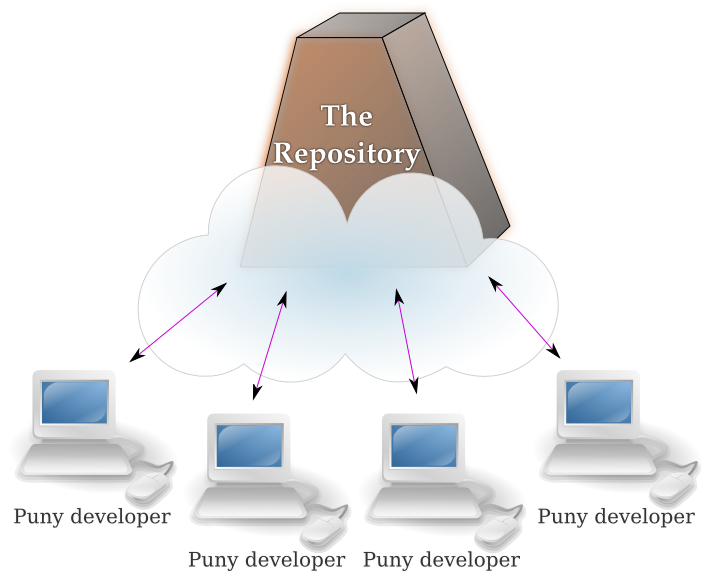
\includegraphics[width=0.9\textwidth]{./images/holy-repo.png}
 \end{figure}
\end{frame}

\begin{frame}{Was bisher so geschah...}{Das Subversion Tagesgeschäft}

  %\begin{itemize}[<+->]
  \begin{itemize}
    \item Zentrales Repository
    \item ``Commitzwang''
    \item Verbindung zum Repository
    \item teure Branches
    \item langsam
  \end{itemize}

\end{frame}

%\begin{frame}[<+->]{Und bei Git?}{}
\begin{frame}{Und bei Git?}{}

  \begin{itemize}
    \item (fast) alles lokal
    \item schnell
    \item klein
    \item kein ``Commitzwang'' (da commits lokal)
    \item verteilt
    \item verschiedene Workflows
    \item billige lokale Branches
  \end{itemize}

\end{frame}

\begin{frame}

  \begin{block}{Erstes Beispiel}
    \begin{itemize}
      \item git init
      \item git clone
      \item git status
      \item git add
      \item git commit
      \item git log
    \end{itemize}
  \end{block} 

\end{frame}

\begin{frame}

 \begin{figure}
  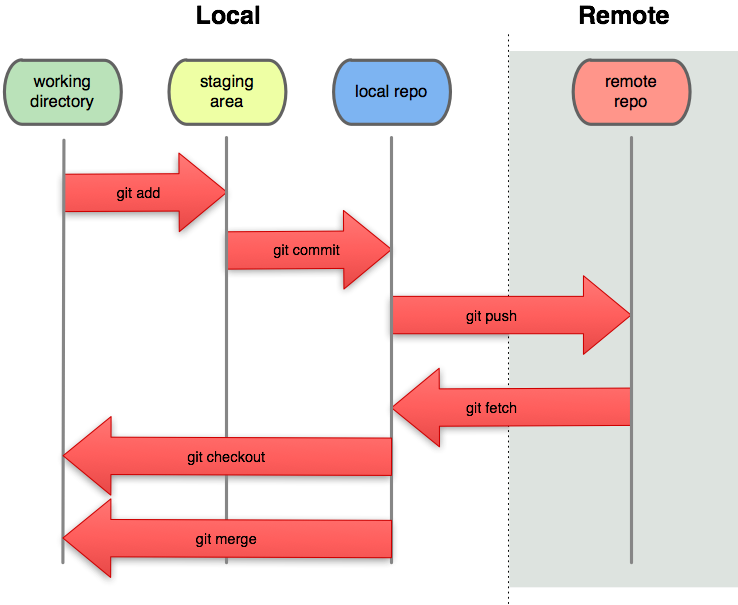
\includegraphics[width=0.90\textwidth]{./images/local-remote.png}
 \end{figure}

\end{frame}

\begin{frame}{SVN vs. Git: Histories}

  \begin{figure}
   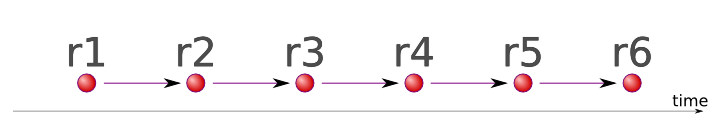
\includegraphics[width=0.95\textwidth]{./images/svn-timeline.png}
  \end{figure}

  \begin{figure}
   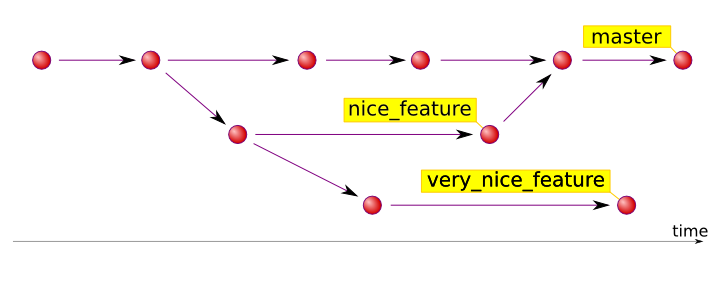
\includegraphics[width=0.95\textwidth]{./images/git-timeline.png}
  \end{figure}

\end{frame}



\begin{frame}{Workflows: Subversion}

  \begin{figure}
     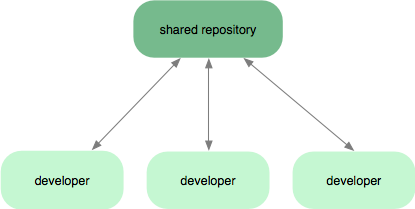
\includegraphics[scale=1.0]{./images/workflow-svn.png}
  \end{figure}

\end{frame}

\begin{frame}{Workflows: Integration Manager}
 
  \begin{figure}
     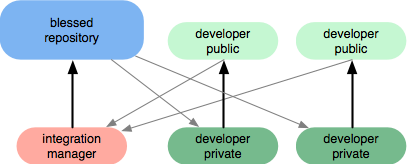
\includegraphics[scale=1.0]{./images/workflow-integration-manager.png}
  \end{figure}

\end{frame}

\begin{frame}{Workflows: Dictator}
 
  \begin{figure}
     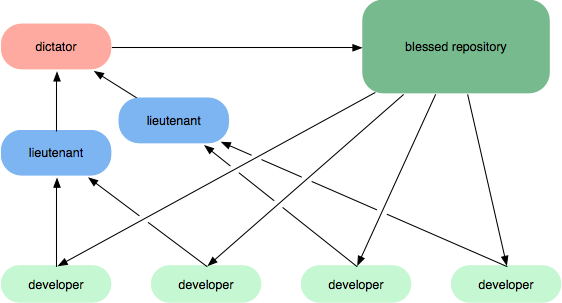
\includegraphics[width=0.95\textwidth]{./images/workflow-dictator.png}
  \end{figure}

\end{frame}


%\begin{frame}[<+->]{Wie alles begann}{}
\begin{frame}{Wie alles begann}{}

  \begin{itemize}
    \item Linux kernel, BitKeeper
    \item Linus Torvalds
    \item Anforderungen: ähnlich wie Bitkeeper, Sicherheit, Effizienz
    \item 2005: Erste Version in 2 Wochen
    \item Wer verwendet Git? Git, Perl, Gnome, Qt, Ruby on Rails, Android, Wine, Fedora, Debian, X.org, VLC, ...
  \end{itemize}

\end{frame}

%\begin{frame}[<+->]{Und sonst so?}{}
\begin{frame}{Und sonst so?}{}

  \begin{itemize}
    \item jedes Objekt SHA1
    \item ``content not files''
    \item Vier Git-Objekte
    \begin{itemize}
     \item blob
     \item tree
     \item commit
     \item tag
    \end{itemize}
  \end{itemize}

\end{frame}

\begin{frame}

  \begin{block}{Branching}
    \begin{itemize}
      \item git branch
      \item git checkout
      \item git merge
    \end{itemize}
  \end{block} 

\end{frame}

%\begin{frame}[<+->]{Git für Fortgeschrittene}{}
\begin{frame}{Git für Fortgeschrittene}{}

  \begin{itemize}
    \item git bisect
    \item git fsck / git gc
    \item git format-patch
    \item git tag v1.0
    \item git blame
    \item git rebase
    \item git cherry-pick
    \item git archive
  \end{itemize}

\end{frame}

%\begin{frame}[<+->]{Kleine Helferlein}{}
\begin{frame}{Kleine Helferlein}{}

  \begin{itemize}
    \item git checkout file.txt
    \item git commit --amend
    \item .gitignore file
    \item gitk (Tk) / qgit (Qt) / gitx (Mac)
    \item git reset --hard \# Vorsicht!
  \end{itemize}

\end{frame}

%\begin{frame}[<+->]{Github.com}
\begin{frame}{Github.com}
\begin{columns}
      \column{.60\textwidth}   
    \begin{itemize}
    \item ``Social Coding", vergleichbar mit Sourceforge
	\item Feb. 2008
	\item 222000 Coder, über 726000 Repositories
	\item Wichtige Projekte
	\begin{itemize}
	  \item Ruby
	  \item Ruby on Rails
	  \item Perl
	  \item PHP
	  \item verschiedene JavaScript-Projekte
	\end{itemize}
  \end{itemize}
\column{.40\textwidth} 
	
\includegraphics[scale=2]{./images/octocat.png}
  \end{columns}
\end{frame}

\begin{frame}
  \Huge{Fragen?}
\end{frame}

\end{document}